\begin{figure}[H]
  \centering
  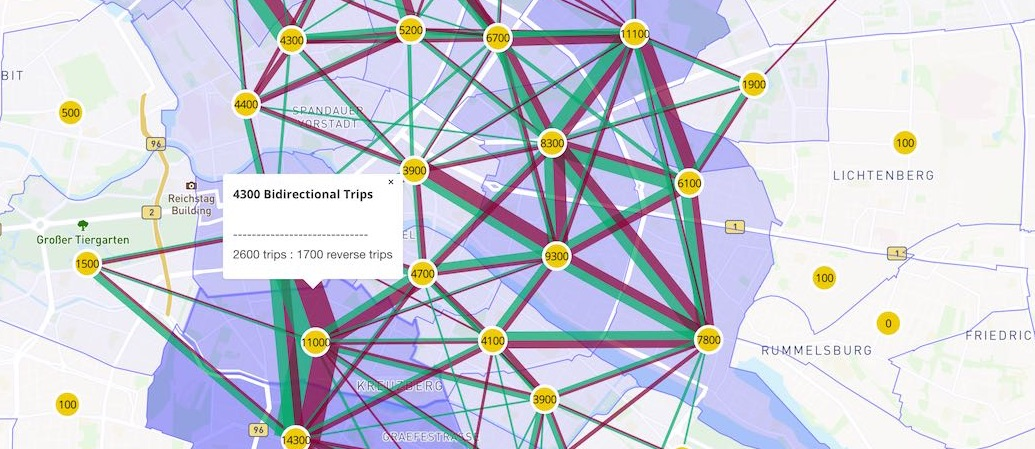
\includegraphics[width=0.8\textwidth]{assets/aggregate-od.jpg}
  \caption{Aggregate Origin/Destination, or ``Spider'' Diagram}
\end{figure}

This visualizion shows aggregated flows between areas defined by a shapefile.
The default view shows everything all at once for every
centroid-to-centroid pair. This can be overwhelming, so you can also
click on an individual centroid to see just the flows to and from that
selected zone.

\hypertarget{usage}{%
\subsection{Usage}}

A file named \texttt{viz-od*.yml} must be present in working folder.
Each yml file matching that pattern will produce a separate Aggregate
O/D diagram.

\textbf{viz-od-example.yml}

\begin{lstlisting}
  # all of the below are required except description and idColumn.
  title: 'My Aggregate Viz'
  description: 'this will be in the sidebar'
  shpFile: Bezirksregionen_zone_GK4_fixed.shp
  dbfFile: Bezirksregionen_zone_GK4_fixed.dbf
  csvFile: od-analysis-hourly-drt.csv
  projection: GK4
  scaleFactor: 100
  idColumn: 'id'
  lineWidth: 50
\end{lstlisting}

\hypertarget{input-files}{%
\subsection{Input Files}}

\textbf{Shapefile:} The DBF data must contain a column with the ID of
the zones/regions. This ID will be used to identify the O/D flows in the
CSV file

\begin{itemize}
\tightlist
\item
  if the \texttt{idColumn} is not specified in YAML then the default
  \texttt{id} will be used.
\item
  If no ID column can be found, then the plot will attempt to use the
  first column in the DBF file.
\end{itemize}

\textbf{O/D CSV File format:}

\begin{itemize}
\tightlist
\item
  Header line contain labels; first two column names will be used for
  from/to (e.g.~origin/destination)
\item
  Column 1: `From' category
\item
  Column 2: `To' category.
\item
  All further columns list flows from/to. For example, there could be 24
  columns, one for each hour of travel
\end{itemize}

\begin{lstlisting}
origin;destination;1;2;3;4;5;6;7;8;9;10;11;12;13;14;15;16;17
88;88;0;0;0;0;0;0;0;0;0;0;0;0;0;0;0;0;0;0;0;0;0;0;0;0
88;89;0;0;0;0;0;0;0;0;0;0;0;0;0;0;0;0;0;0;0;0;0;0;0;0
88;110;0;0;0;0;0;0;0;0;0;0;0;0;0;0;0;0;0;0;0;0;0;0;0;0
88;111;0;0;0;0;0;0;0;0;0;0;0;0;0;0;0;0;0;0;0;0;0;0;0;0
88;112;0;0;0;0;0;0;0;0;0;0;0;0;0;0;0;0;0;0;0;0;0;0;0;0
etc...
\end{lstlisting}

\hypertarget{configuration-parameters}{%
\subsection{Configuration Parameters}\label{configuration-parameters}}

\textbf{projection:} Coordinate projection, such as ``EPSG:31468'' or
``GK4''

\textbf{scaleFactor:} Factor to scale all values -- to handle 1\% or
10\% scenarios, for example

\textbf{lineWidth:} Starting width scaling of lines

\textbf{idColumn:} Data column in shapefile which contains the ID for
regions/zones (default ``id'')
